\documentclass[12pt,a4paper]{article}

% ---------- Core packages ----------
\usepackage[a4paper,left=1.25in,right=1in,top=1in,bottom=1in]{geometry}
\usepackage{mathptmx}
\usepackage[T1]{fontenc}
\usepackage[utf8]{inputenc}
\usepackage{microtype}
\usepackage{graphicx}
\usepackage{xcolor}
\usepackage{titlesec}
\usepackage{fancyhdr}
\usepackage{booktabs}
\usepackage{array}
\usepackage{longtable}
\usepackage{enumitem}
\usepackage{tikz}
\usetikzlibrary{positioning,arrows.meta}
\usepackage{setspace}
\usepackage{hyperref}
\usepackage{float}
\usepackage{amssymb}

% ---------- Brand colours (match the app + thesis) ----------
\definecolor{brandprimary}{HTML}{0E7C86}
\definecolor{branddark}{HTML}{0B4F57}
\definecolor{brandgray}{HTML}{374151}

\hypersetup{
    colorlinks=true, linkcolor=branddark, citecolor=branddark, urlcolor=brandprimary,
    pdftitle={Project Proposal: LLM-Orchestrated Retrieval-Augmented Conversational Agent for Cross-Platform Product Discovery, Semantic Matching and Personalized E-Commerce Recommendation},
    pdfauthor={Tanvir Ahmed},
}

\titleformat{\section}{\normalfont\Large\bfseries\color{branddark}}{\thesection}{0.6em}{}
\titleformat{\subsection}{\normalfont\large\bfseries\color{brandgray}}{\thesubsection}{0.6em}{}
\titlespacing*{\section}{0pt}{18pt}{8pt}

\pagestyle{fancy}
\fancyhf{}
\setlength{\headheight}{14pt}
\renewcommand{\headrulewidth}{0.4pt}
\fancyhead[L]{\small\itshape ShopMate AI --- LLM-Orchestrated Retrieval-Augmented Shopping Agent}
\fancyhead[R]{\small\itshape Tanvir Ahmed}
\fancyfoot[C]{\thepage}
\fancypagestyle{plain}{\fancyhf{}\fancyfoot[C]{\thepage}\renewcommand{\headrulewidth}{0pt}}

\graphicspath{{figures/}}
\newcommand{\xmark}{$\times$}
\emergencystretch=3em
\tolerance=1200
\hbadness=10000

\begin{document}

% ============================================================
% TITLE PAGE
% ============================================================
\begin{titlepage}
\centering
\vspace*{0.2cm}
{\bfseries\fontsize{14}{16}\selectfont Mawlana Bhashani Science and Technology University}\\[3pt]
{\small Santosh, Tangail-1902, Bangladesh}\\[14pt]

\includegraphics[height=2.1cm]{mbstu-logo.png}

\vspace{12pt}
{\bfseries\fontsize{12}{14}\selectfont Department of Information and Communication Technology}\\[22pt]

{\color{brandprimary}\rule{0.82\textwidth}{0.8pt}}\\[7pt]
{\bfseries\fontsize{15}{18}\selectfont\color{branddark} PROJECT PROPOSAL}\\[7pt]
{\color{brandprimary}\rule{0.82\textwidth}{0.8pt}}\\[22pt]

{\bfseries\fontsize{16}{19}\selectfont ShopMate AI}\\[10pt]
\begin{minipage}{0.82\textwidth}
\centering
{\bfseries\fontsize{12.5}{16}\selectfont Design and Development of an LLM-Orchestrated, Retrieval-Augmented Conversational Agent for Cross-Platform Product Discovery, Semantic Product Matching and Personalized E-Commerce Recommendation\par}
\end{minipage}\\[24pt]

{\small Submitted in partial fulfilment of the requirements for the degree of}\\[3pt]
{\bfseries\fontsize{11.5}{14}\selectfont Master of Engineering in Information and Communication Technology}\\[32pt]

\begin{minipage}{0.42\textwidth}
\centering
\small\textbf{Submitted by}\\[6pt]
\normalsize\textbf{Tanvir Ahmed}\\
\small Student ID: IT22604\\
M.Engineering (ICT)
\end{minipage}%
\begin{minipage}{0.42\textwidth}
\centering
\small\textbf{Submitted to}\\[6pt]
\normalsize\textbf{Nazrul Islam}\\
\small Associate Professor\\
Department of ICT\\
MBSTU

\end{minipage}

\vfill
{\normalsize\itshape August 2026}
\end{titlepage}

% ============================================================
\section{Introduction}

Online shopping in Bangladesh, as elsewhere, has grown into a fragmented experience: a buyer who wants a single
product often has to open several e-commerce sites, repeat the same search on each, and manually compare price,
delivery cost, seller reliability and reviews before deciding where to buy. This proposal outlines a project to
design, develop, and evaluate \textbf{ShopMate AI}, an LLM-orchestrated, retrieval-augmented conversational agent
that lets a user describe what they need in natural language --- including Bengali and Banglish --- and have the
system perform transformer-based intent/entity extraction, hybrid dense-vector and keyword retrieval, cross-store
semantic product matching, and learning-to-rank-style personalized recommendation across multiple supported
stores, from a single conversational interface.

\section{Background and Motivation}

Conventional e-commerce search is keyword-driven: it matches the literal words in a query against product titles
and returns an unranked or popularity-ranked list, leaving the buyer to open each store separately, re-type the
same search, and manually reconcile differences in price, delivery charge, seller rating and stock status.
Constraint-rich, natural requests such as ``a black backpack under BDT 3,000 that can carry both a laptop and
clothes'' are handled poorly by keyword search, and code-mixed Bengali-English queries are often not understood at
all. Recent progress in transformer-based language understanding, sentence embeddings and semantic retrieval makes
it practical to build a conversational agent that extracts structured shopping requirements from free-form text,
matches semantically equivalent products across stores, and produces an explainable, ranked recommendation. This
project is motivated by that gap between what buyers actually want to say and what current shopping interfaces are
able to understand.

\section{Problem Statement}

Specifically, the absence of a conversational, cross-platform shopping agent leaves buyers without:
\begin{itemize}[leftmargin=1.3cm]
    \item A single interface through which a natural-language or Bangla/Banglish shopping request can be
    understood and acted on;
    \item An automated way to identify the \emph{same or equivalent} product listed under different titles and
    descriptions across stores;
    \item A structured, explainable comparison of price, delivery cost, seller quality, rating and availability
    across supported stores;
    \item A mechanism to be notified when a tracked product's price drops or a desired item is restocked; and
    \item A human-confirmed, safe purchase or redirect workflow rather than either fully manual shopping or
    unsupervised automated checkout.
\end{itemize}

\section{Objectives}

\subsection{General Objective}
To design, implement, and evaluate a modular, LLM-orchestrated, retrieval-augmented conversational shopping agent
that understands natural-language (including Bangla/Banglish) shopping requests, searches supported e-commerce
sources through hybrid dense-vector and keyword retrieval, performs transformer-based semantic product matching
and comparison, generates personalized, explainable recommendations via a learning-to-rank-style scoring model,
monitors prices and stock, and supports human-confirmed purchasing workflows.

\subsection{Specific Objectives}
\begin{enumerate}[leftmargin=1.3cm]
    \item Design a service-oriented architecture that separates business logic (Laravel) from AI/NLP processing
    (Python FastAPI service).
    \item Implement an intent-classification and entity-extraction pipeline capable of parsing English,
    Bengali and code-mixed shopping queries into structured requirements (product, brand, budget, quantity,
    colour, size, rating threshold, delivery preference).
    \item Build a hybrid keyword + semantic retrieval pipeline over a normalized, multi-store product catalogue
    using sentence embeddings and a vector-capable store.
    \item Implement cross-store semantic product matching so that the same or equivalent product listed under
    different titles is correctly identified and compared.
    \item Implement a hybrid, explainable ranking and recommendation engine that combines relevance, price,
    rating, delivery, seller quality and availability, with a stated reason for each recommendation.
    \item Implement price-drop and restock alerting, and a shopping-list module for recurring purchases.
    \item Implement a human-confirmed order/redirect workflow, using only official APIs, affiliate feeds or
    permitted integrations, with no automated bypass of authentication, CAPTCHA or payment controls.
    \item Evaluate the system experimentally against conventional keyword-based search using Precision@K,
    Recall@K, NDCG@K, product-matching accuracy, search time, task completion and user satisfaction.
\end{enumerate}

\section{Scope of the Project}

The project scope covers conversational product discovery, cross-store comparison, personalized recommendation,
and price/stock monitoring, delivered as a modular web application (Laravel + Python FastAPI AI service) with one
or two permitted store integrations for the MVP. The following are explicitly \textbf{out of scope} for the
initial delivery, and are identified instead as future/advanced work: full automated purchase execution without
human confirmation; voice shopping and visual (image-based) product search; SMS gateway integration; and coverage
of more than a small number of store integrations. Automated bypass of CAPTCHA, authentication, anti-bot measures
or payment security is explicitly excluded from the design at every stage.

\section{Literature Review Summary}

A review of existing approaches --- native e-commerce site search, third-party price-comparison sites, and
general-purpose conversational shopping assistants --- shows a consistent gap for a buyer in the Bangladeshi
market: native site search is keyword-only and cannot compare across stores; price-comparison sites are typically
manually curated, updated infrequently, and do not understand natural-language or Bangla/Banglish constraints; and
published conversational-commerce research largely targets English-only, single-market catalogues rather than the
multilingual, code-mixed, multi-store setting relevant here. This project is positioned to close that specific
gap: a conversational agent combining intent/entity extraction, semantic product matching and explainable,
multi-factor ranking, evaluated specifically on Bangla/Banglish and multi-constraint shopping queries against a
conventional keyword-search baseline.

\section{Proposed System Architecture}

The system will follow a modular, service-oriented architecture that isolates AI/NLP processing from core business
logic, as shown in Figure~\ref{fig:arch}.

\begin{figure}[H]
\centering
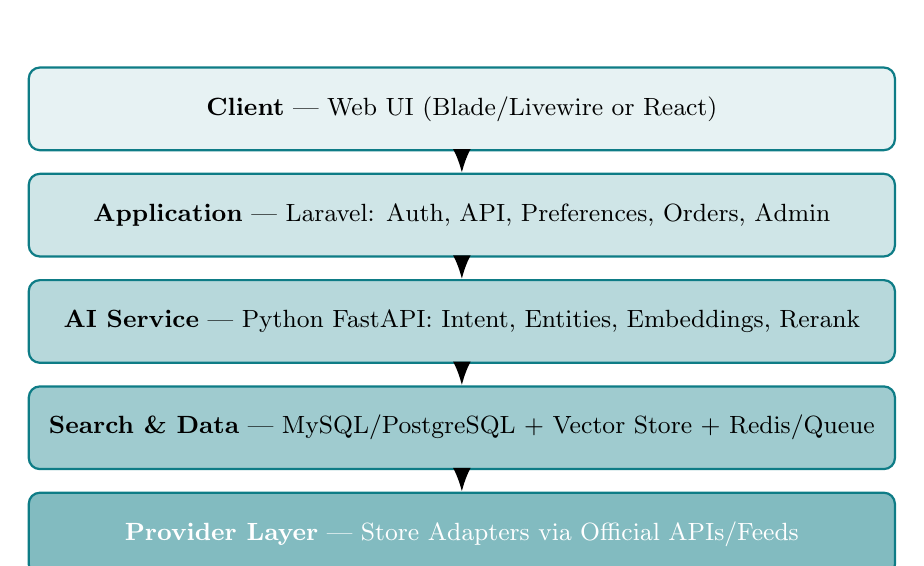
\begin{tikzpicture}[
    layer/.style={draw, rounded corners, minimum width=11cm, minimum height=1.05cm, align=center, font=\small},
    every path/.style={-{Latex[length=3mm]}, thick}
]
    \node[layer, fill=brandprimary!10, draw=brandprimary] (client) at (0,6.3) {\textbf{Client} --- Web UI (Blade/Livewire or React)};
    \node[layer, fill=brandprimary!20, draw=brandprimary] (app) at (0,4.95) {\textbf{Application} --- Laravel: Auth, API, Preferences, Orders, Admin};
    \node[layer, fill=brandprimary!30, draw=brandprimary] (ai) at (0,3.6) {\textbf{AI Service} --- Python FastAPI: Intent, Entities, Embeddings, Rerank};
    \node[layer, fill=brandprimary!40, draw=brandprimary] (data) at (0,2.25) {\textbf{Search \& Data} --- MySQL/PostgreSQL + Vector Store + Redis/Queue};
    \node[layer, fill=brandprimary!52, draw=brandprimary, text=white] (provider) at (0,0.9) {\textbf{Provider Layer} --- Store Adapters via Official APIs/Feeds};
    \draw (client) -- (app);
    \draw (app) -- (ai);
    \draw (ai) -- (data);
    \draw (data) -- (provider);
\end{tikzpicture}
\caption{Proposed layered, service-oriented architecture}
\label{fig:arch}
\end{figure}

Laravel owns authentication, business logic, user data, orders and the administrative dashboard; it communicates
with the Python AI service over an internal API for intent detection, entity extraction, embeddings, semantic
search, reranking and review analysis. Store-specific adapters implement a common provider interface
(\texttt{searchProducts()}, \texttt{getProduct()}, \texttt{getAvailability()}, \texttt{getPrice()},
\texttt{getDeliveryInfo()}, \texttt{getReviews()}, and, where officially supported, \texttt{createOrder()},
\texttt{cancelOrder()}, \texttt{trackOrder()}), so the AI/search layer remains independent of any particular
e-commerce site and new stores can be added without changing core application logic.

\section{Proposed Modules}

Table~\ref{tab:modules} summarises the twelve functional modules proposed for this system.

\begin{longtable}{p{3.6cm}p{9.8cm}}
\caption{Proposed functional modules} \label{tab:modules} \\
\toprule
\textbf{Module} & \textbf{Description} \\
\midrule
\endfirsthead
\toprule
\textbf{Module} & \textbf{Description} \\
\midrule
\endhead
User Management & Registration, login, profile, addresses, preferences and privacy controls. \\
Conversational Interface & Chat UI, conversation history, context management and command parsing. \\
Intent \& Entity Engine & Classify intent and extract product, brand, budget, quantity, colour, size and other constraints. \\
Product Search & Keyword + semantic/hybrid search across the normalized product catalogue. \\
Product Matching & Match equivalent products across stores using embeddings, attributes and reranking. \\
Price Comparison & Normalize price, discount, delivery charge and availability for comparison. \\
Review Intelligence & Collect permitted reviews and generate sentiment/topic summaries. \\
Recommendation Engine & Combine content similarity, user preferences and purchase/search history into a ranked, explained result. \\
Shopping List & Create, edit, schedule and recommend recurring shopping items. \\
Alerts & Price-drop, stock-restock and scheduled-purchase notifications. \\
Order Management & Order creation/redirect, status tracking and cancellation where supported. \\
Admin Dashboard & Store health, products, users, AI confidence, search analytics and system statistics. \\
\bottomrule
\end{longtable}

\section{Tools and Technologies}

\begin{table}[H]
\centering
\caption{Proposed technology stack}
\begin{tabular}{ll}
\toprule
\textbf{Layer} & \textbf{Technology} \\
\midrule
Backend framework & Laravel (PHP), REST API \\
Frontend & Laravel Blade/Livewire or React/Vue; responsive web UI \\
AI service & Python + FastAPI \\
AI / NLP & Hugging Face Transformers: sentence embeddings, rerankers, instruction-following LLM \\
Database & MySQL or PostgreSQL (transactional data) \\
Vector search & pgvector, Qdrant or Weaviate \\
Cache / queue & Redis + Laravel Queue / Celery \\
Search & Elasticsearch/OpenSearch or hybrid vector + keyword search \\
Deployment & Ubuntu Linux + Docker + Nginx + HTTPS \\
Monitoring & Application logs, health checks, optional Prometheus/Grafana \\
\bottomrule
\end{tabular}
\end{table}

\section{Proposed Methodology}

The system will be developed incrementally, module by module, following a repeatable per-module cycle: (1) design
the data schema and API contract for the module; (2) implement the Laravel side (migration, model, controller,
routes, views) and, where relevant, the corresponding FastAPI endpoint; (3) integrate with the store provider
layer using seeded or sandbox product data; (4) evaluate the AI components of the module (intent accuracy, entity
F1, retrieval quality, ranking quality) against a held-out query set; and (5) document the milestone before
proceeding to the next module. AI model selection will be evidence-based: candidate embedding, classification,
entity-extraction, reranking and LLM-orchestration models will be benchmarked on English, Bengali and code-mixed
queries, and for each candidate the model name, version, parameter size, latency, memory requirement, license,
evaluation dataset and measured accuracy will be recorded so that the final model choice is reproducible.

\section{AI Pipeline}

\noindent\textbf{Step 1 --- Query Understanding:} Normalize the user message and detect language/code-mixed text.\\
\textbf{Step 2 --- Intent Classification:} Map the message to intents such as \texttt{SEARCH\_PRODUCT},
\texttt{COMPARE\_PRODUCT}, \texttt{BUY\_PRODUCT}, \texttt{TRACK\_ORDER}, \texttt{PRICE\_ALERT},
\texttt{STOCK\_ALERT}, \texttt{RECOMMEND\_PRODUCT} or \texttt{SHOPPING\_LIST}.\\
\textbf{Step 3 --- Requirement Extraction:} Extract entities such as category, brand, model, budget, quantity,
colour, size, rating threshold and delivery preference.\\
\textbf{Step 4 --- Retrieval:} Perform hybrid keyword + vector retrieval over the unified product catalogue.\\
\textbf{Step 5 --- Product Matching:} Calculate semantic similarity and compare structured attributes to identify
equivalent products across stores.\\
\textbf{Step 6 --- Ranking:} Combine relevance, price, rating, delivery, seller quality, availability and user
preference into a ranking score.\\
\textbf{Step 7 --- Recommendation:} Generate an explanation such as ``Best overall'', ``Lowest price'', ``Fastest
delivery'' or ``Best rated''.\\
\textbf{Step 8 --- Action:} If the user requests an order, require explicit confirmation before any supported
purchase or checkout-redirect action.

\section{Database Design}

\noindent\textbf{Main tables:} users, user\_preferences, addresses, stores, products, product\_variants,
product\_images, store\_products, product\_prices, product\_availability, reviews, review\_analysis,
conversations, messages, search\_history, product\_views, shopping\_lists, shopping\_list\_items, price\_alerts,
stock\_alerts, orders, order\_items, order\_status\_history and recommendations.

\noindent\textbf{Vector collections:} product embeddings, review embeddings and, optionally, user-interest
embeddings. Store identifiers and product source URLs are preserved in every record for traceability back to the
originating store.

\section{Security and Privacy}

\begin{itemize}[leftmargin=1.3cm]
    \item Use HTTPS everywhere and secure API authentication between Laravel and the AI service.
    \item Encrypt sensitive user data at rest where appropriate.
    \item Use role-based access control for users, administrators and provider operators.
    \item Never expose merchant credentials or payment information to the LLM or AI service.
    \item Apply prompt-injection and tool-use safeguards to the conversational shopping agent.
    \item Validate all product/provider responses before they reach the user.
    \item Keep audit logs for AI decisions, order actions and administrative changes.
    \item Use only official APIs, affiliate feeds or permitted integrations; do not design around bypassing
    CAPTCHA, authentication or anti-bot measures.
    \item Require mandatory human confirmation before any real purchase; do not store payment credentials unless
    a compliant payment architecture is explicitly designed.
\end{itemize}

\section{Testing Plan}

\begin{longtable}{p{3.6cm}p{9.8cm}}
\toprule
\textbf{Test Area} & \textbf{Examples} \\
\midrule
\endfirsthead
\toprule
\textbf{Test Area} & \textbf{Examples} \\
\midrule
\endhead
Unit Testing & Laravel services, AI response parsers, ranking functions, provider adapters. \\
API Testing & Authentication, search, product details, alerts, orders and AI-service integration. \\
AI Evaluation & Intent accuracy, entity-extraction F1, semantic retrieval quality, product-matching and reranking accuracy. \\
Recommendation Testing & Precision@K, Recall@K, NDCG@K and user-preference alignment. \\
Performance Testing & Search latency, concurrent users, queue throughput and provider response handling. \\
Security Testing & Authentication, authorization, injection, data exposure and API abuse. \\
User Acceptance Testing & Realistic shopping tasks with representative users, including Bangla/Banglish queries. \\
\bottomrule
\end{longtable}

\section{MSc Research Evaluation}

\noindent\textbf{Research Question:} Can a conversational AI agent improve product discovery and purchasing
efficiency across multiple Bangladeshi e-commerce platforms compared with conventional keyword-based shopping?

\noindent\textbf{Baseline:} Conventional keyword-based product search with manually compared results.

\noindent\textbf{Experimental System:} ShopMate AI with semantic retrieval, cross-store product matching and
personalized, explainable ranking.

\noindent\textbf{Evaluation:} A controlled set of shopping queries covering budget, brand, attribute,
ambiguous-name, Bangla/Banglish and multi-constraint requests will be used to compare relevance, search time, task
completion, product-matching accuracy and user satisfaction between the baseline and the experimental system. The
thesis will report datasets, model configurations, evaluation methodology, quantitative results, limitations and
error analysis.

\section{Work Plan and Timeline}

Table~\ref{tab:timeline} presents the proposed development schedule, grouped into four phases across twenty weeks.

\begin{table}[H]
\centering
\caption{Proposed work plan}
\label{tab:timeline}
\begin{tabular}{p{2.6cm}p{3.3cm}p{7.0cm}}
\toprule
\textbf{Phase} & \textbf{Duration} & \textbf{Activities} \\
\midrule
Phase 1 & Weeks 1--4 & Requirements analysis, literature review, architecture, dataset design, Laravel foundation, authentication, database and admin panel. \\
Phase 2 & Weeks 5--10 & First store/provider integration and product ingestion; intent classification, entity extraction and conversational API; embeddings, semantic search, product matching and reranking. \\
Phase 3 & Weeks 11--16 & Price comparison, recommendation engine, review intelligence, shopping lists, price/stock alerts, human-confirmed purchase/redirect workflow and security hardening. \\
Phase 4 & Weeks 17--20 & Testing, performance optimization, research experiments, user study, analysis, documentation and thesis writing. \\
\bottomrule
\end{tabular}
\end{table}

\begin{figure}[H]
\centering
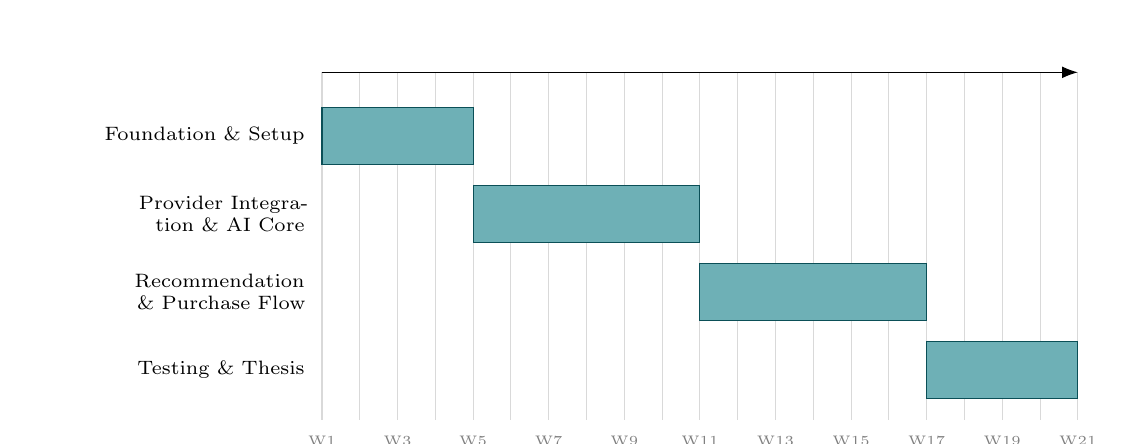
\begin{tikzpicture}[y=0.9cm, x=0.48cm]
    \foreach \x in {1,...,21} {
        \draw[gray!30] (\x,-4.6) -- (\x,0.3);
    }
    \foreach \x in {1,3,5,7,9,11,13,15,17,19,21} {
        \node[font=\tiny, gray] at (\x,-4.9) {W\x};
    }
    \draw[-{Latex[length=2mm]}] (1,0.3) -- (21,0.3);

    \draw[fill=brandprimary!60, draw=branddark] (1,-1.0) rectangle (5,-0.2);
    \node[anchor=east, font=\scriptsize, text width=3.4cm, align=right] at (0.8,-0.6) {Foundation \& Setup};

    \draw[fill=brandprimary!60, draw=branddark] (5,-2.1) rectangle (11,-1.3);
    \node[anchor=east, font=\scriptsize, text width=3.4cm, align=right] at (0.8,-1.7) {Provider Integration \& AI Core};

    \draw[fill=brandprimary!60, draw=branddark] (11,-3.2) rectangle (17,-2.4);
    \node[anchor=east, font=\scriptsize, text width=3.4cm, align=right] at (0.8,-2.8) {Recommendation \& Purchase Flow};

    \draw[fill=brandprimary!60, draw=branddark] (17,-4.3) rectangle (21,-3.5);
    \node[anchor=east, font=\scriptsize, text width=3.4cm, align=right] at (0.8,-3.9) {Testing \& Thesis};
\end{tikzpicture}
\caption{Proposed 20-week project timeline (Gantt overview)}
\label{fig:gantt}
\end{figure}

\section{MVP vs.\ Advanced Scope}

\noindent\textbf{MVP:} One or two permitted store integrations, conversational product search, semantic matching,
price comparison, recommendation, product links, user preferences and basic alerts.

\noindent\textbf{Advanced:} Multiple providers, review intelligence, SMS/voice interfaces, visual search,
personalized learning, price history, recurring shopping and supported order automation.

\noindent\textbf{Future Research:} Multi-agent shopping, learning-to-rank, reinforcement from user feedback,
broader marketplace coverage and autonomous purchase planning under strict human approval.

\section{Expected Outcome}

The final system should demonstrate that a user can express a shopping need conversationally --- in English or
Bangla/Banglish --- and receive relevant, explainable, cross-platform product options without manually visiting
multiple websites. The system is expected to reduce search and comparison effort while providing measurable
improvements in product relevance and task completion relative to conventional keyword search.

\noindent\textbf{Final Deliverables:} working web application, AI service, normalized product/search pipeline,
provider adapter framework, database, admin dashboard, evaluation dataset, experimental results, documentation,
deployment setup and MSc thesis/presentation materials.

\section{References}
\begin{enumerate}[leftmargin=1.3cm]
    \item T.~Mikolov et al., ``Distributed Representations of Words and Phrases and their Compositionality,'' in
    \textit{Advances in Neural Information Processing Systems (NeurIPS)}, 2013, pp.~3111--3119.
    \item N.~Reimers and I.~Gurevych, ``Sentence-BERT: Sentence Embeddings using Siamese BERT-Networks,'' in
    \textit{Proc. EMNLP-IJCNLP}, 2019, pp.~3982--3992.
    \item J.~Devlin et al., ``BERT: Pre-training of Deep Bidirectional Transformers for Language Understanding,''
    in \textit{Proc. NAACL-HLT}, 2019, pp.~4171--4186.
    \item C.~D. Manning, P.~Raghavan, and H.~Sch\"utze, \textit{Introduction to Information Retrieval}. Cambridge
    University Press, 2008.
    \item OWASP Foundation, ``OWASP Top Ten Web Application Security Risks,'' 2021.
    \url{https://owasp.org/www-project-top-ten/}
    \item Laravel LLC, ``Laravel Documentation.'' \url{https://laravel.com/docs}
    \item Hugging Face, ``Transformers Documentation.'' \url{https://huggingface.co/docs/transformers}
    \item FastAPI, ``FastAPI Documentation.'' \url{https://fastapi.tiangolo.com}
\end{enumerate}

\end{document}
